\documentclass[12pt,a4paper,twoside]{report}
% -------------------------------------------------------------------- %
% Pacotes

\usepackage[utf8]{inputenc}
\usepackage[T1]{fontenc}
\usepackage[brazil]{babel}
\usepackage[fixlanguage]{babelbib}
\usepackage[pdftex]{graphicx}      % usamos arquivos pdf/png como figuras
\usepackage{setspace}              % espaçamento flexvel
\usepackage{indentfirst}           % indentação do primeiro parágrafo
\usepackage{makeidx}               % índice remissivo
\usepackage[nottoc]{tocbibind}     % acrescentamos a bibliografia/indice/conteudo no Table of Contents
\usepackage{courier}               % usa o Adobe Courier no lugar de Computer Modern Typewriter
\usepackage{type1cm}               % fontes realmente escaláveis
\usepackage{titletoc}
\usepackage{ucs}
\usepackage[font=small,format=plain,labelfont=bf,up,textfont=it,up]{caption}
\usepackage[usenames,svgnames,dvipsnames]{xcolor}
\usepackage[a4paper,top=2.54cm,bottom=2.0cm,left=2.0cm,right=2.54cm]{geometry} % margens
\usepackage{amsmath}
\usepackage{booktabs} % cria tabelas em formato profissional
\usepackage[pdftex,plainpages=false,pdfpagelabels,pagebackref,colorlinks=true,citecolor=DarkGreen,
linkcolor=NavyBlue,urlcolor=DarkRed,filecolor=green,bookmarksopen=true]{hyperref} % links coloridos
\usepackage[all]{hypcap}                % soluciona o problema com o hyperref e capítulos
\usepackage[square,sort,nonamebreak,comma]{natbib}  % citação bibliográfica alpha
\fontsize{60}{62}\usefont{OT1}{cmr}{m}{n}{\selectfont}
\usepackage{upquote}                    % formata apóstrofes '
\usepackage{textcomp}

% Para formatar corretamente as URLs
\usepackage{url}
% -------------------------------------------------------------------- %
% Cabeçalhos similares ao TAOCP de Donald E. Knuth
\usepackage{fancyhdr}
\pagestyle{fancy}
\fancyhf{}
\renewcommand{\chaptermark}[1]{\markboth{\MakeUppercase{#1}}{}}
\renewcommand{\sectionmark}[1]{\markright{\MakeUppercase{#1}}{}}
\renewcommand{\headrulewidth}{0pt}

\frenchspacing                     % arruma o espaço: id est (i.e.) e exempli gratia (e.g.)
\urlstyle{same}                    % URL com o mesmo estilo do texto e no mono-spaced
\makeindex                         % para o índice remissivo
\raggedbottom                      % para no permitir espaços extras no texto
\fontsize{60}{62}\usefont{OT1}{cmr}{m}{n}{\selectfont}
\cleardoublepage
\normalsize

% -------------------------------------------------------------------- %
% Cores para formatação de código
\usepackage{color}
\definecolor{vermelho}{rgb}{0.6,0,0} % para strings
\definecolor{verde}{rgb}{0.25,0.5,0.35} % para comentários
\definecolor{roxo}{rgb}{0.5,0,0.35} % para palavras-chaves
\definecolor{azul}{rgb}{0.25,0.35,0.75} % para strings
\definecolor{cinza-claro}{gray}{0.95}
% -------------------------------------------------------------------- %
% Opções de listagem usados para o código fonte
% Ref: http://en.wikibooks.org/wiki/LaTeX/Packages/Listings
\usepackage{listings}           % para formatar código-fonte (ex. em Java)

\lstset{ %
language=Python,                      % seleciona a linguagem do código
basicstyle=\footnotesize\ttfamily,    % o tamanho da fonte usado no código
commentstyle=\color{verde}\bfseries,  % formatação de comentários
stringstyle=\color{azul},             % formatação de strings
upquote=true,
numbers=left,                   % onde colocar os números de linha
numberstyle=\tiny,  % o tamanho da fonte usada para a numeração das linhas
stepnumber=1,                   % o intervalo entre dois números de linhas. Se for 1, numera cada uma.
numbersep=5pt,                  % how far the line-numbers are from the code
showspaces=false,               % show spaces adding particular underscores
showstringspaces=false,         % underline spaces within strings
showtabs=false,                 % show tabs within strings adding particular underscores
keywordstyle=\color{roxo}\bfseries,
keywordstyle=[1]\color{roxo}\bfseries,
keywordstyle=[2]\color{verde}\bfseries,
frame=b,                   % adds a frame around the code
framerule=0.6pt,
tabsize=2,                      % sets default tabsize to 2 spaces
captionpos=t,                   % sets the caption-position to top
breaklines=true,                % sets automatic line breaking
breakatwhitespace=false,        % sets if automatic breaks should only happen at whitespace
escapeinside={\%*}{*)},         % if you want to add a comment within your code
backgroundcolor=\color[rgb]{1.0,1.0,1.0}, % choose the background color.
rulecolor=\color[rgb]{0.8,0.8,0.8},
extendedchars=true,
xleftmargin=10pt,
xrightmargin=10pt,
framexleftmargin=10pt,
framexrightmargin=10pt,
literate={â}{{\^{a}}}1  % para formatar corretamente os acentos do Português ao usar utf8
    {ê}{{\^{e}}}1
    {ô}{{\^{o}}}1
    {Â}{{\^{A}}}1
    {Ê}{{\^{E}}}1
    {Ô}{{\^{O}}}1
    {á}{{\'{a}}}1
    {é}{{\'{e}}}1
    {í}{{\'{i}}}1
    {ó}{{\'{o}}}1
    {ú}{{\'{u}}}1
    {Á}{{\'{A}}}1
    {É}{{\'{E}}}1
    {Í}{{\'{I}}}1
    {Ó}{{\'{O}}}1
    {Ú}{{\'{U}}}1
    {à}{{\`{a}}}1
    {À}{{\`{A}}}1
    {ã}{{\~{a}}}1
    {õ}{{\~{o}}}1
    {Ã}{{\~{A}}}1
    {Õ}{{\~{O}}}1
    {ç}{{\c{c}}}1
    {Ç}{{\c{C}}}1
    {ü}{{\"u}}1
    {Ü}{{\"U}}1
}

\renewcommand{\lstlistingname}{Listagem}
\renewcommand{\lstlistlistingname}{Lista de Listagens}

% \captionsetup[lstlisting]{singlelinecheck=false, labelfont={blue}, textfont={blue}}
\usepackage{caption}
\DeclareCaptionFont{white}{\color{white}}
\DeclareCaptionFormat{listing}{\colorbox[cmyk]{0.43, 0.35, 0.35,0.01}{\parbox{\textwidth}{\hspace{15pt}#1#2#3}}}
\captionsetup[lstlisting]{format=listing,labelfont=white,textfont=white, singlelinecheck=false, margin=0pt, font={bf,footnotesize}}

\title{Análise experimental de algoritmos usando Python}
\author{Patrícia Mariana Ramos Marcolino \\
\texttt{\small \url{pmrmarcolino@hotmail.com}}
\vspace{1cm} \\
Eduardo Pinheiro Barbosa \\
\texttt{\small \url{eduardptu@hotmail.com}}
\vspace{1cm} \\
Faculdade de Computação \\
Universidade Federal de Uberlândia
}
\date{\today}

\begin{document}
\maketitle
% -------------------------------------------------------------------- %
% Listas de figuras, tabelas e códigos criadas automaticamente
\listoffigures
\listoftables
\lstlistoflistings
% -------------------------------------------------------------------- %

% -------------------------------------------------------------------- %
% Sumário
\tableofcontents
% cabeçalho para as páginas de todos os capítulos
\fancyhead[RE,LO]{\thesection}

%\singlespacing              % espaçamento simples
\setlength{\parskip}{0.15in} % espaçamento entre paragráfos
\chapter{Análise}

O algoritmo não faz comparações entre elementos de A.
Sua complexidade deve ser medida com base nas outras
operações (aritméticas, atribuições, etc.)
Claramente, o número de tais operações é uma função em
$O(n + k)$, já que temos dois loops simples com n iterações
e dois com k iterações.
 Assim, quando $k ∈ O(n)$, este algoritmo tem complexidade
$O(n)$.


\chapter{Resultados}
\section{Tabelas}

\input{../countingsort/tabelas/countingsortAleatorio.tex}

\begin{figure}[ht]
\centering 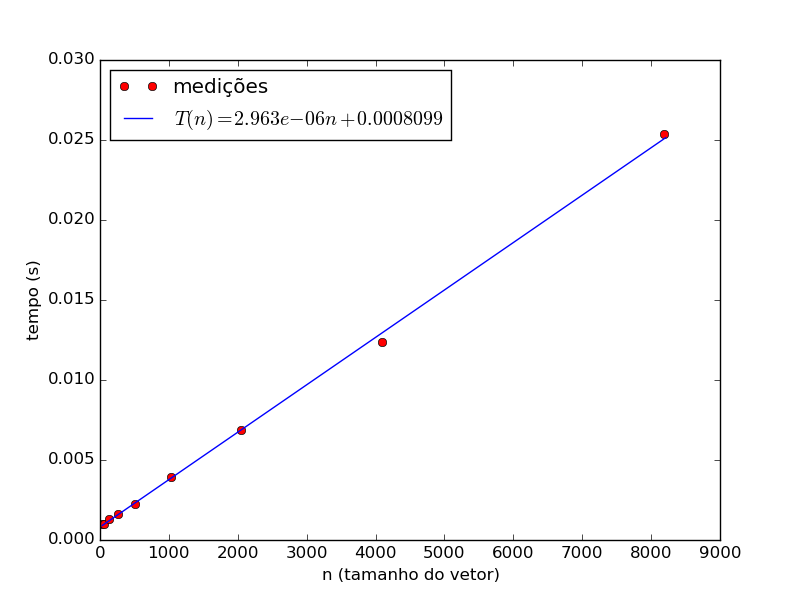
\includegraphics[scale=0.8]{../countingsort/imagens/countingsortAleatorio0.png}
\caption{A análise do grafico para $2^{32}$ segue abaixo para countingsort}

Tendo a função $T(n) = 2.963\mathrm{e}-6*n-0.0008099$ e para o $n =2^{32}$, $T(2^{32}) = 12725.987288148$ 
\label{fig:countingsortAleatorio0}
\end{figure}

\begin{figure}[ht]
\centering 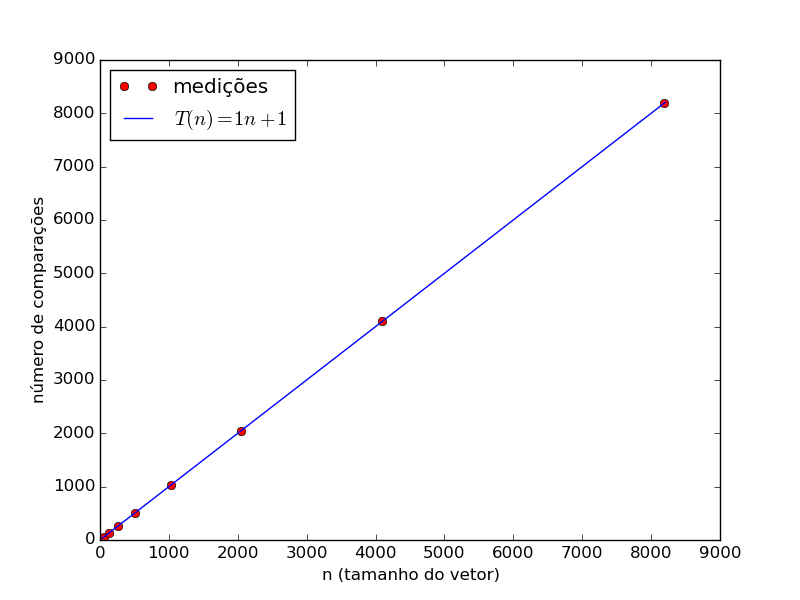
\includegraphics[scale=0.8]{../countingsort/imagens/countingsortAleatorio1.png}
\caption{A análise do grafico para $2^{32}$ segue abaixo para countingsort}

Tendo a função $T(n) = n+1 $ e para o $n =2^{32}$, $T(2^{32}) = 4294967297$ 
\label{fig:countingsortAleatorio1}
\end{figure}


\input{../countingsort/tabelas/countingsortCrescente.tex}

\begin{figure}[ht]
\centering 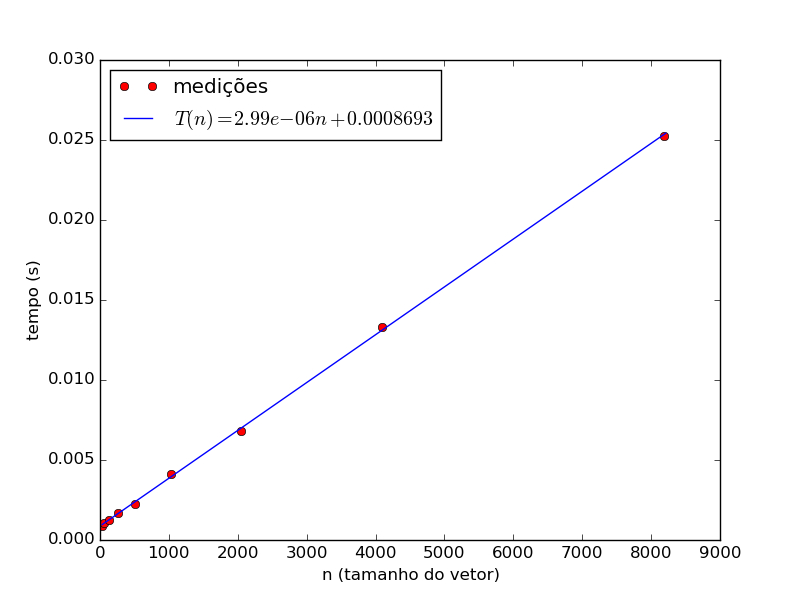
\includegraphics[scale=0.8]{../countingsort/imagens/countingsortCrescente0.png}
\caption{A análise do grafico para $2^{32}$ segue abaixo para countingsort}

Tendo a função $T(n) = 2.99\mathrm{e}-6*n-0.0008693$ e para o $n =2^{32}$, $T(2^{32}) = 12841.95134574$ 
\label{fig:countingsortCrescente0}
\end{figure}

\begin{figure}[ht]
\centering 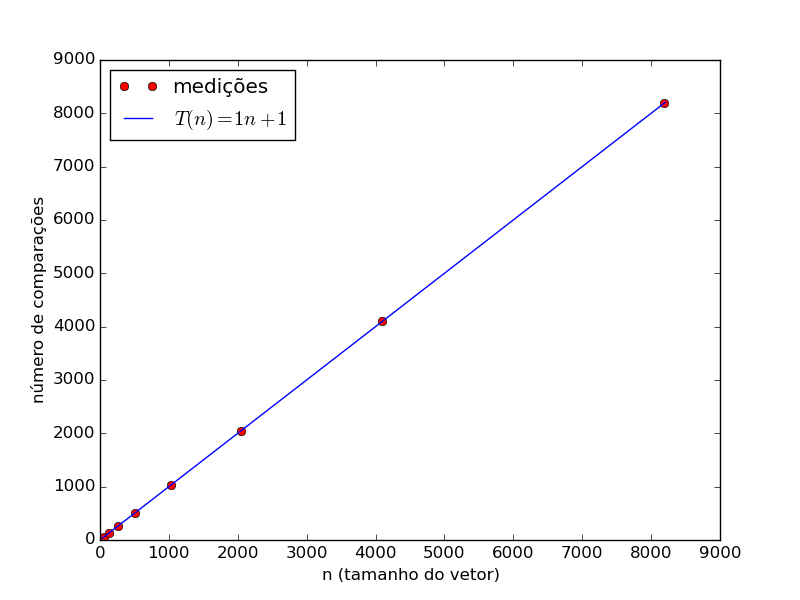
\includegraphics[scale=0.8]{../countingsort/imagens/countingsortCrescente1.png}
\caption{A análise do grafico para $2^{32}$ segue abaixo para countingsort}

Tendo a função $T(n) = n+1 $ e para o $n =2^{32}$, $T(2^{32}) = 4294967297 $ 
\label{fig:countingsortCrescente1}
\end{figure}


\input{../countingsort/tabelas/countingsortDecrescente.tex}

\begin{figure}[ht]
\centering 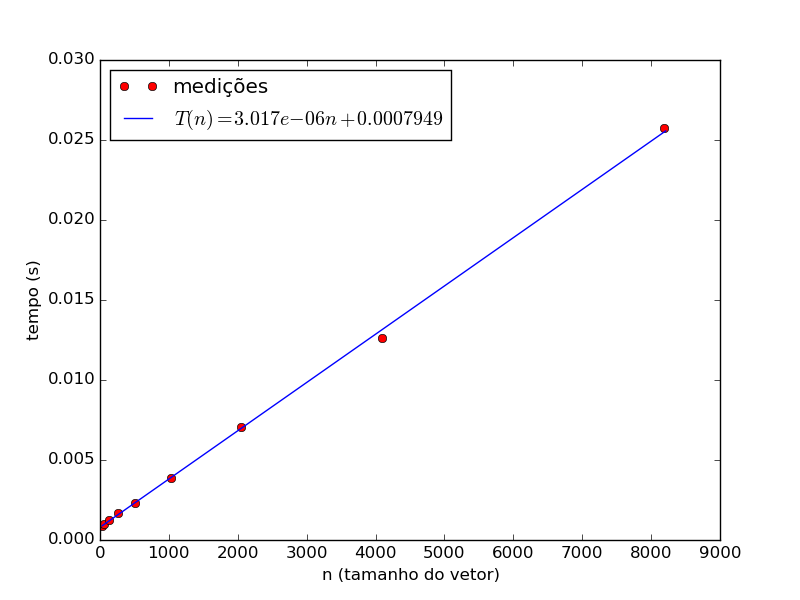
\includegraphics[scale=0.8]{../countingsort/imagens/countingsortDecrescente0.png}
\caption{A análise do grafico para $2^{32}$ segue abaixo para countingsort}

Tendo a função $T(n) = 3.017\mathrm{e}-6*n-0.0007949$ e para o $n =2^{32}$, $T(2^{32}) = 12957.915537132$ 
\label{fig:countingsortDecrescente0}
\end{figure}

\begin{figure}[ht]
\centering 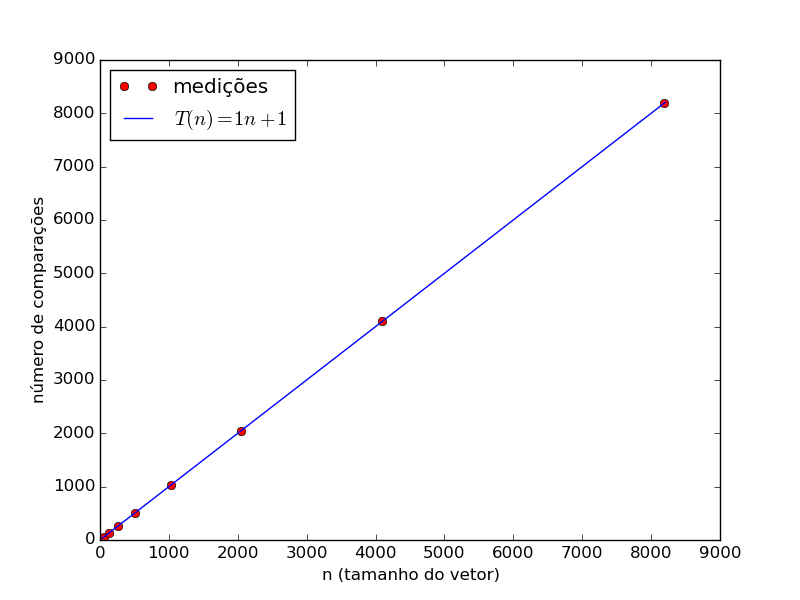
\includegraphics[scale=0.8]{../countingsort/imagens/countingsortDecrescente1.png}
\caption{A análise do grafico para $2^{32}$ segue abaixo para countingsort}

Tendo a função $T(n) = n+1 $ e para o $n =2^{32}$, $T(2^{32}) = 4294967297$ 
\label{fig:countingsortDecrescente1}
\end{figure}


\input{../countingsort/tabelas/countingsortQuaseCresc10.tex}

\begin{figure}[ht]
\centering 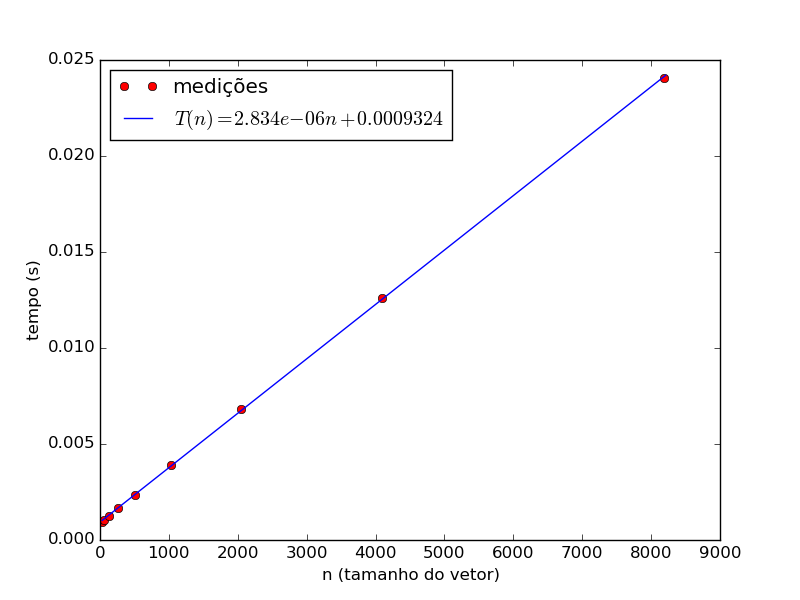
\includegraphics[scale=0.8]{../countingsort/imagens/countingsortQuaseCresc100.png}
\caption{A análise do grafico para $2^{32}$ segue abaixo para countingsort}

Tendo a função $T(n) = 2.834\mathrm{e}-6*n-0.0009324$ e para o $n =2^{32}$, $T(2^{32}) = 12171.936384464$ 
\label{fig:countingsortQuaseCresc100}
\end{figure}

\begin{figure}[ht]
\centering 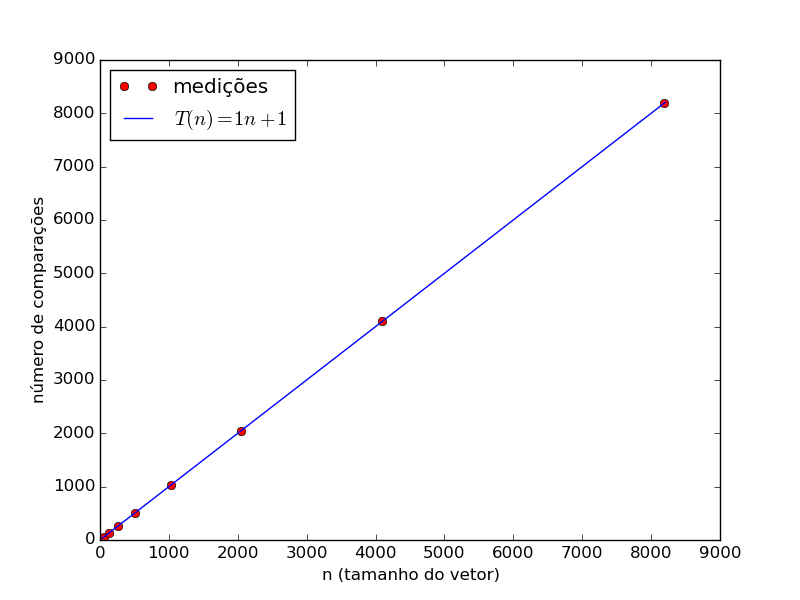
\includegraphics[scale=0.8]{../countingsort/imagens/countingsortQuaseCresc101.png}
\caption{A análise do grafico para $2^{32}$ segue abaixo para countingsort}

Tendo a função $T(n) = n+1 $ e para o $n =2^{32}$, $T(2^{32}) = 4294967297$ 
\label{fig:countingsortQuaseCresc101}
\end{figure}


\input{../countingsort/tabelas/countingsortQuaseCresc20.tex}

\begin{figure}[ht]
\centering 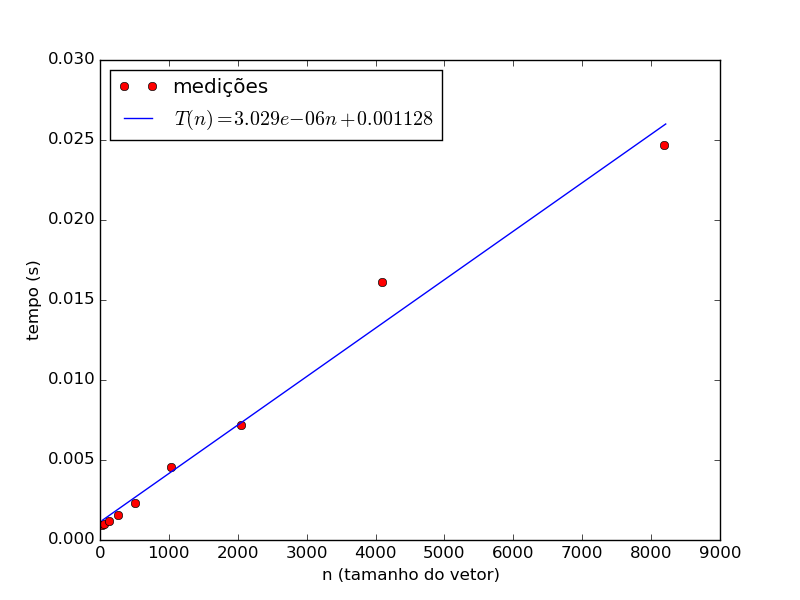
\includegraphics[scale=0.8]{../countingsort/imagens/countingsortQuaseCresc200.png}
\caption{A análise do grafico para $2^{32}$ segue abaixo para countingsort}

Tendo a função $T(n) = 3.029\mathrm{e}-6*n-0.0001128$ e para o $n =2^{32}$, $T(2^{32}) = 13009.455826784$ 
\label{fig:countingsortQuaseCresc200}
\end{figure}

\begin{figure}[ht]
\centering 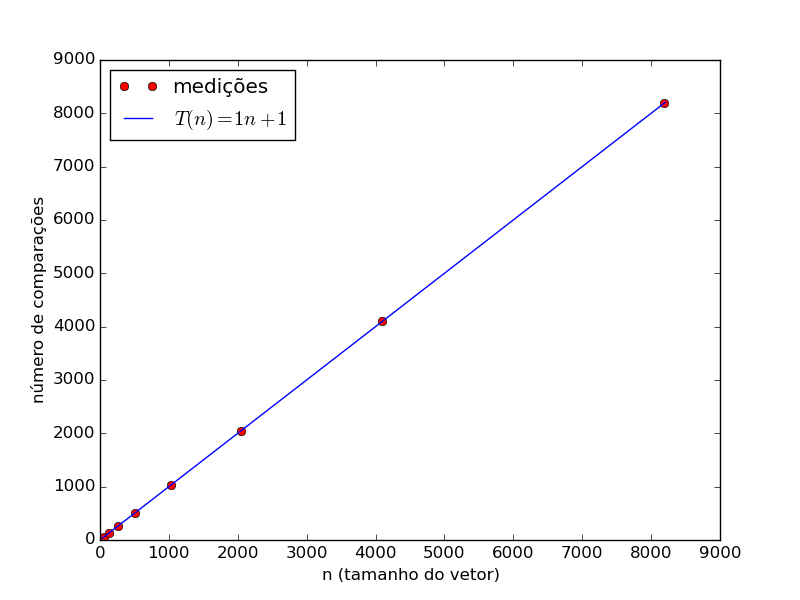
\includegraphics[scale=0.8]{../countingsort/imagens/countingsortQuaseCresc201.png}
\caption{A análise do grafico para $2^{32}$ segue abaixo para countingsort}

Tendo a função $T(n) =n+1$ e para o $n =2^{32}$, $T(2^{32}) = 4294967297$ 
\label{fig:countingsortQuaseCresc201}
\end{figure}

\clearpage
\input{../countingsort/tabelas/countingsortQuaseCresc30.tex}

\begin{figure}[ht]
\centering 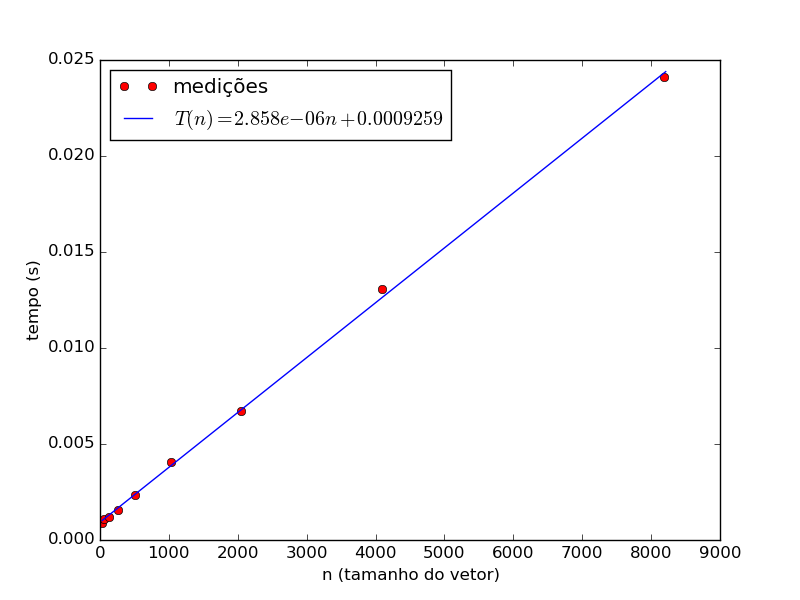
\includegraphics[scale=0.8]{../countingsort/imagens/countingsortQuaseCresc300.png}
\caption{A análise do grafico para $2^{32}$ segue abaixo para countingsort}

Tendo a função $T(n) = 2.858\mathrm{e}-6*n-0.0009259$ e para o $n =2^{32}$, $T(2^{32}) = 12275.015606068$ 
\label{fig:countingsortQuaseCresc300}
\end{figure}

\begin{figure}[ht]
\centering 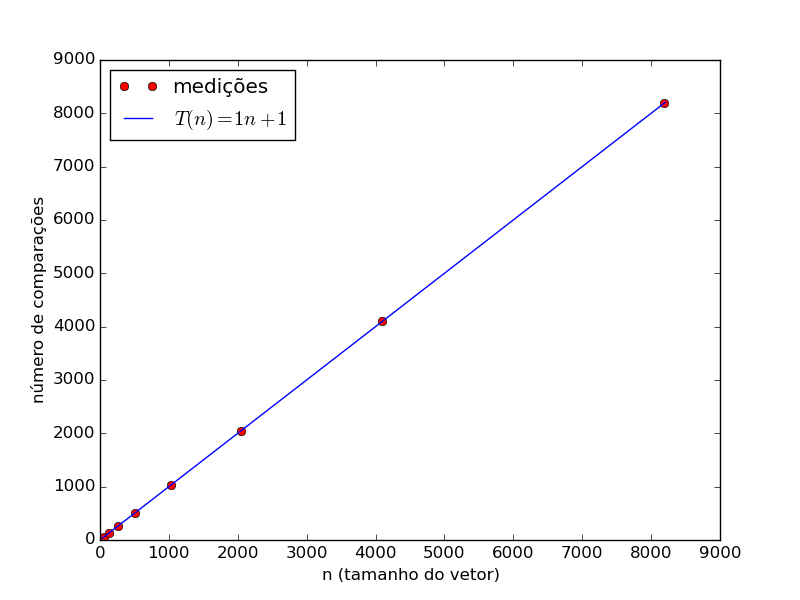
\includegraphics[scale=0.8]{../countingsort/imagens/countingsortQuaseCresc301.png}
\caption{A análise do grafico para $2^{32}$ segue abaixo para countingsort}

Tendo a função $T(n) = n+1 $ e para o $n =2^{32}$, $T(2^{32}) = 4294967297$ 
\label{fig:countingsortQuaseCresc301}
\end{figure}


\input{../countingsort/tabelas/countingsortQuaseCresc40.tex}

\begin{figure}[ht]
\centering 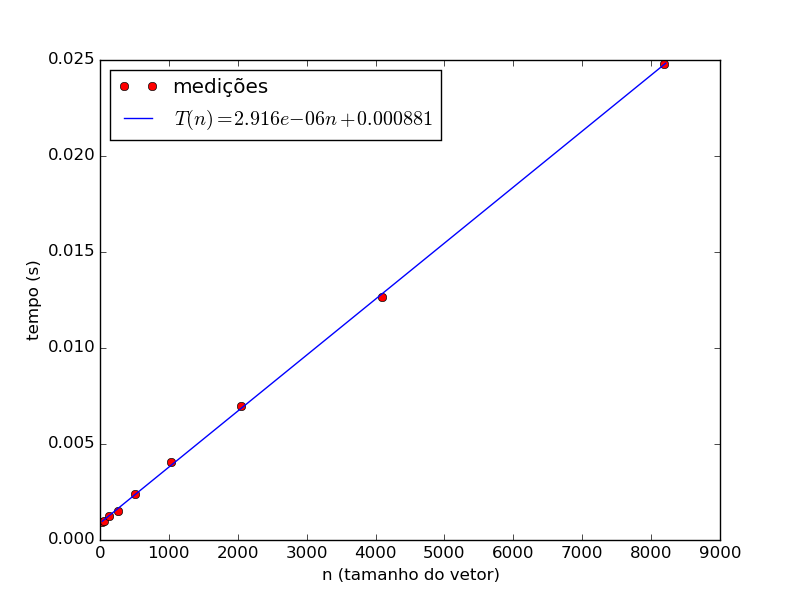
\includegraphics[scale=0.8]{../countingsort/imagens/countingsortQuaseCresc400.png}
\caption{A análise do grafico para $2^{32}$ segue abaixo para countingsort}

Tendo a função $T(n) = 2.916\mathrm{e}-6*n-0.000881$ e para o $n =2^{32}$, $T(2^{32}) = 12524.123754136$ 
\label{fig:countingsortQuaseCresc400}
\end{figure}

\begin{figure}[ht]
\centering 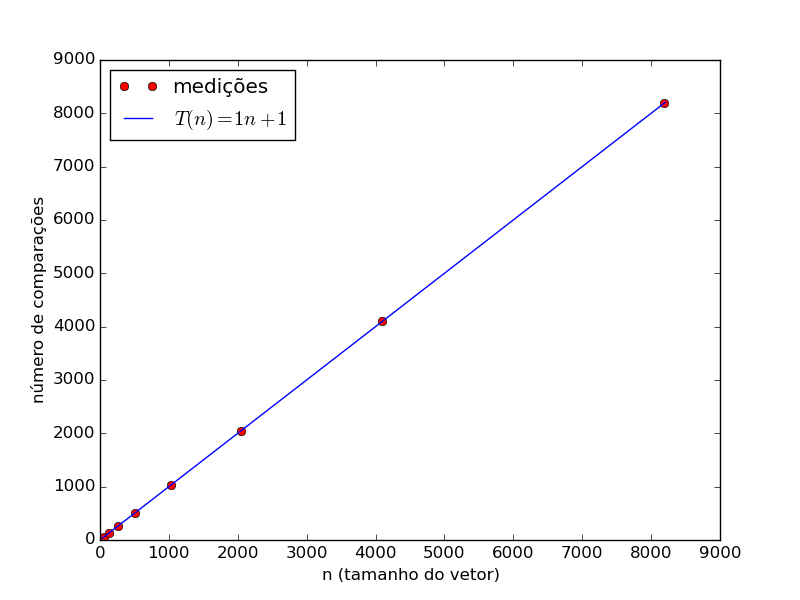
\includegraphics[scale=0.8]{../countingsort/imagens/countingsortQuaseCresc401.png}
\caption{A análise do grafico para $2^{32}$ segue abaixo para countingsort}

Tendo a função $T(n) = n+1$ e para o $n =2^{32}$, $T(2^{32}) = 4294967297$ 
\label{fig:countingsortQuaseCresc401}
\end{figure}


\input{../countingsort/tabelas/countingsortQuaseCresc50.tex}

\begin{figure}[ht]
\centering 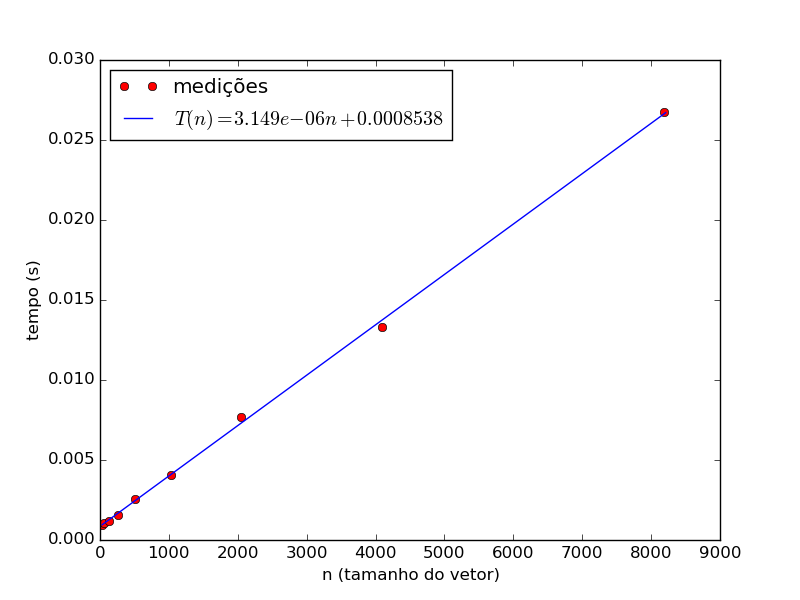
\includegraphics[scale=0.8]{../countingsort/imagens/countingsortQuaseCresc500.png}
\caption{A análise do grafico para $2^{32}$ segue abaixo para countingsort}

Tendo a função $T(n) = 3.149\mathrm{e}-6*n-0.0008538$ e para o $n =2^{32}$, $T(2^{32}) = 13524.851161304$ 
\label{fig:countingsortQuaseCresc500}
\end{figure}

\begin{figure}[ht]
\centering 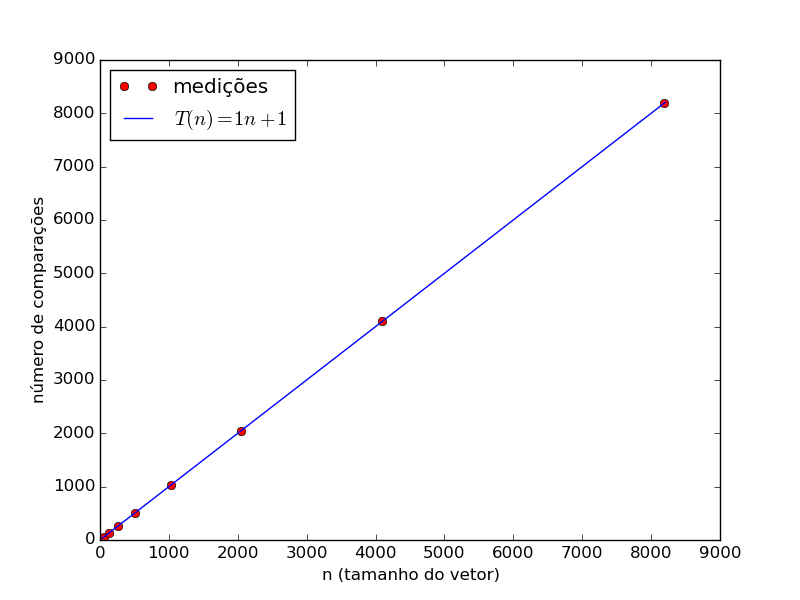
\includegraphics[scale=0.8]{../countingsort/imagens/countingsortQuaseCresc501.png}
\caption{A análise do grafico para $2^{32}$ segue abaixo para countingsort}

Tendo a função $T(n) = n+1$ e para o $n =2^{32}$, $T(2^{32}) = 4294967297$ 
\label{fig:countingsortQuaseCresc501}
\end{figure}


\input{../countingsort/tabelas/countingsortQuaseDecresc10.tex}

\begin{figure}[ht]
\centering 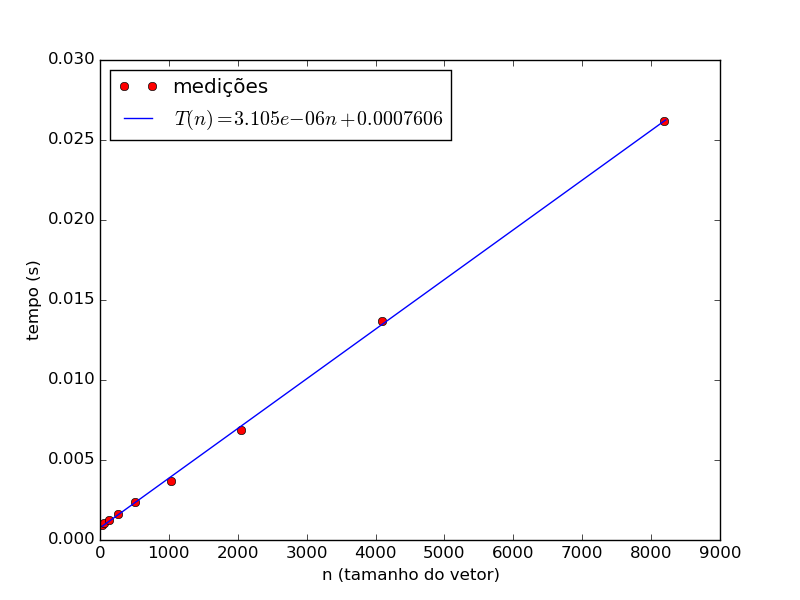
\includegraphics[scale=0.8]{../countingsort/imagens/countingsortQuaseDecresc100.png}
\caption{A análise do grafico para $2^{32}$ segue abaixo para countingsort}

Tendo a função $T(n) = 3.105\mathrm{e}-6*n-0.0007606$ e para o $n =2^{32}$, $T(2^{32}) = 13335.87269348$ 
\label{fig:countingsortQuaseDecresc100}
\end{figure}

\begin{figure}[ht]
\centering 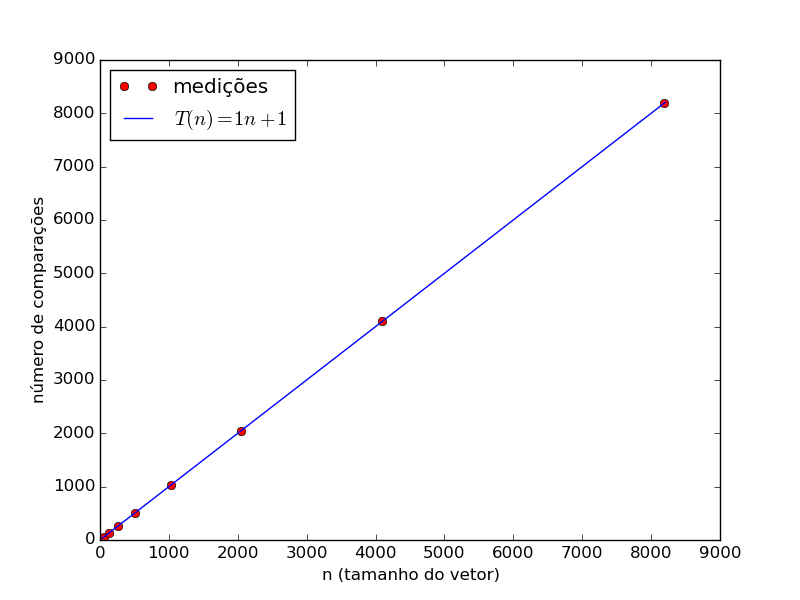
\includegraphics[scale=0.8]{../countingsort/imagens/countingsortQuaseDecresc101.png}
\caption{A análise do grafico para $2^{32}$ segue abaixo para countingsort}

Tendo a função $T(n) = n+1$ e para o $n =2^{32}$, $T(2^{32}) = 4294967297$ 
\label{fig:countingsortQuaseDecresc101}
\end{figure}


\input{../countingsort/tabelas/countingsortQuaseDecresc20.tex}

\begin{figure}[ht]
\centering 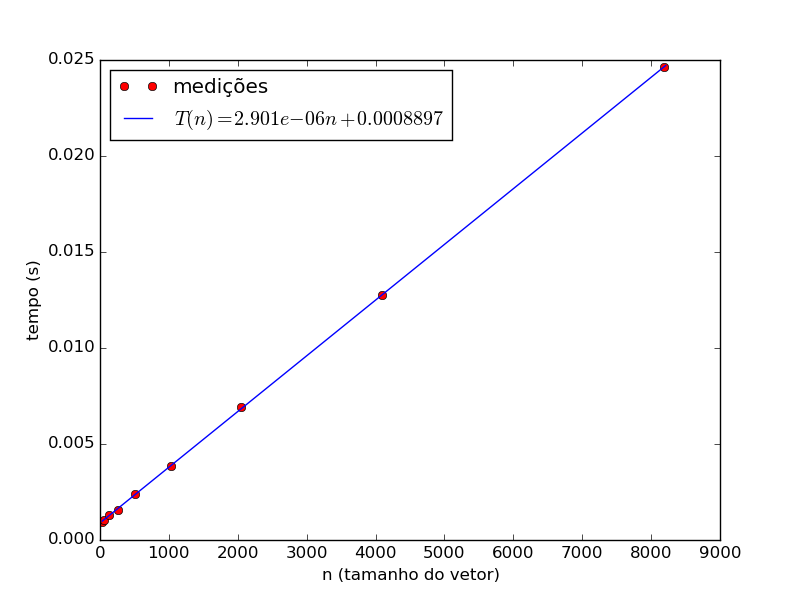
\includegraphics[scale=0.8]{../countingsort/imagens/countingsortQuaseDecresc200.png}
\caption{A análise do grafico para $2^{32}$ segue abaixo para countingsort}

Tendo a função $T(n) = 2.901\mathrm{e}-6*n-0.0008897$ e para o $n =2^{32}$, $T(2^{32}) = 12459.699235996$ 
\label{fig:countingsortQuaseDecresc200}
\end{figure}

\begin{figure}[ht]
\centering 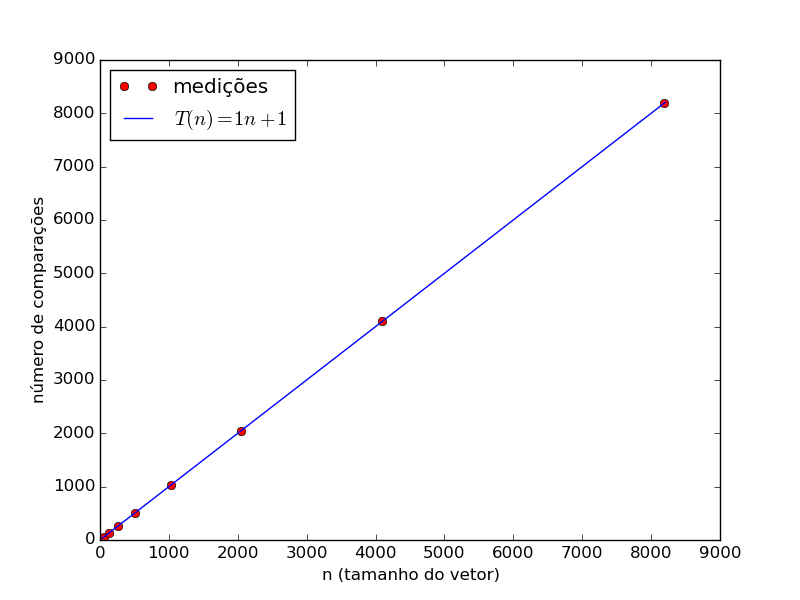
\includegraphics[scale=0.8]{../countingsort/imagens/countingsortQuaseDecresc201.png}
\caption{A análise do grafico para $2^{32}$ segue abaixo para countingsort}

Tendo a função $T(n) = n+1$ e para o $n =2^{32}$, $T(2^{32}) = 4294967297$ 
\label{fig:countingsortQuaseDecresc201}
\end{figure}

\clearpage
\input{../countingsort/tabelas/countingsortQuaseDecresc30.tex}

\begin{figure}[ht]
\centering 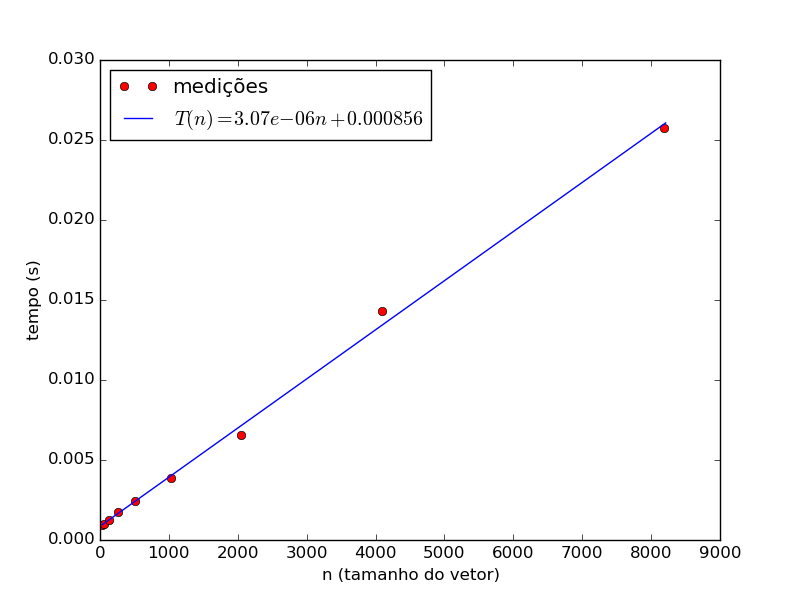
\includegraphics[scale=0.8]{../countingsort/imagens/countingsortQuaseDecresc300.png}
\caption{A análise do grafico para $2^{32}$ segue abaixo para countingsort}

Tendo a função $T(n) = 3.07\mathrm{e}-6*n-0.000856$ e para o $n =2^{32}$, $T(2^{32}) = 13185.54874272$ 
\label{fig:countingsortQuaseDecresc300}
\end{figure}

\begin{figure}[ht]
\centering 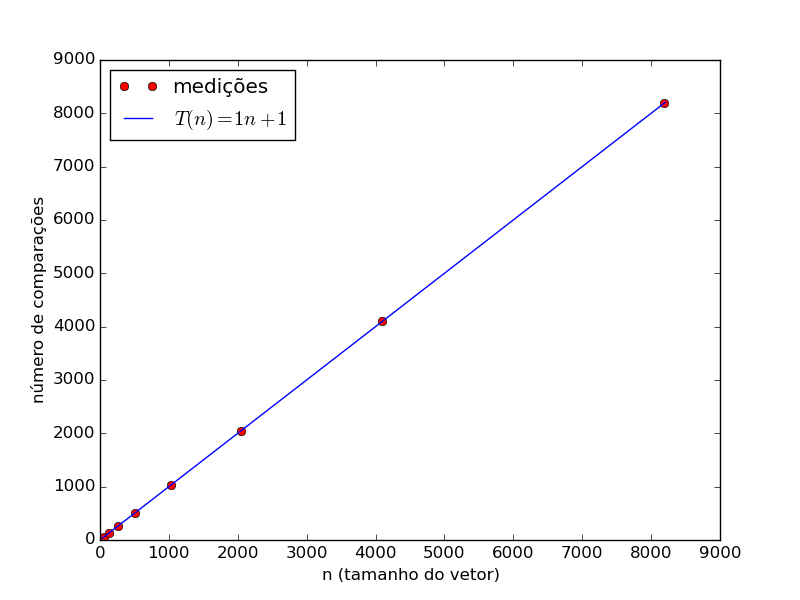
\includegraphics[scale=0.8]{../countingsort/imagens/countingsortQuaseDecresc301.png}
\caption{A análise do grafico para $2^{32}$ segue abaixo para countingsort}

Tendo a função $T(n) = n+1$ e para o $n =2^{32}$, $T(2^{32}) = 4294967297$ 
\label{fig:countingsortQuaseDecresc301}
\end{figure}


\input{../countingsort/tabelas/countingsortQuaseDecresc40.tex}

\begin{figure}[ht]
\centering 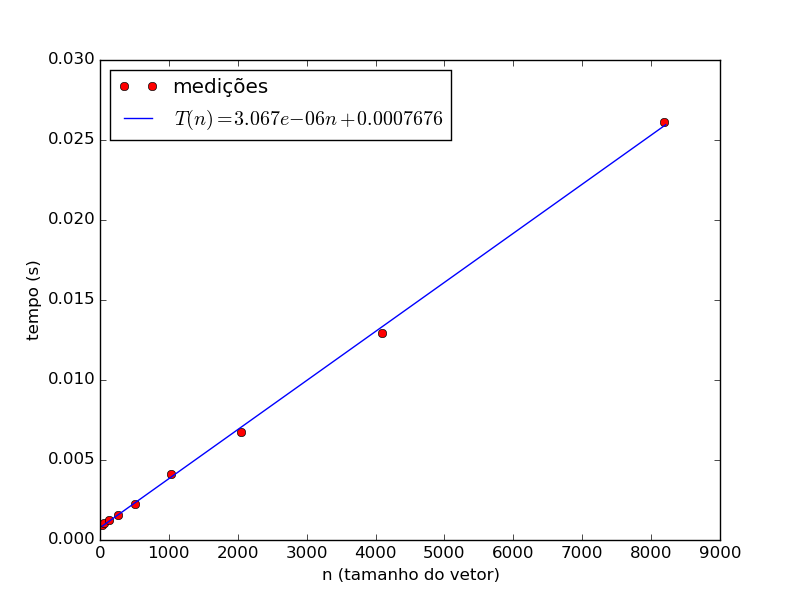
\includegraphics[scale=0.8]{../countingsort/imagens/countingsortQuaseDecresc400.png}
\caption{A análise do grafico para $2^{32}$ segue abaixo para countingsort}

Tendo a função $T(n) = 3.067\mathrm{e}-6*n-0.0007676$ e para o $n =2^{32}$, $T(2^{32}) = 13172.663929232$ 
\label{fig:countingsortQuaseDecresc400}
\end{figure}

\begin{figure}[ht]
\centering 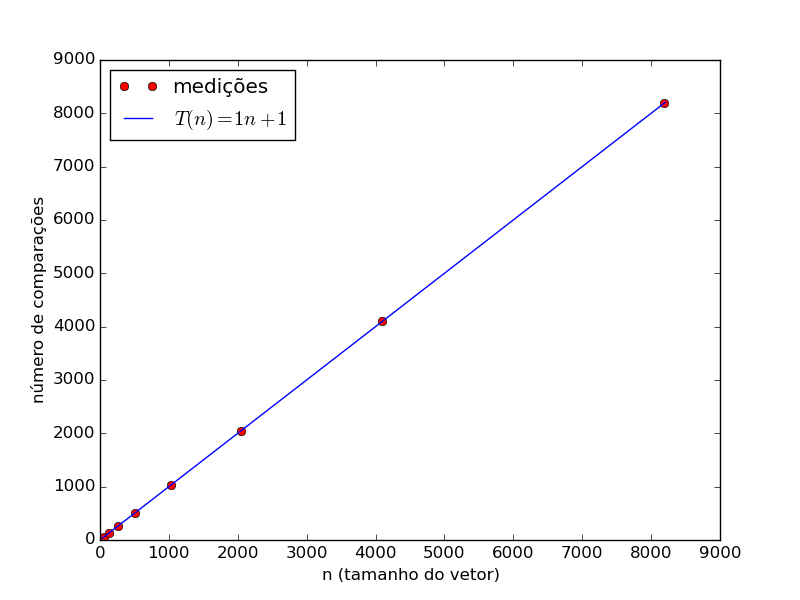
\includegraphics[scale=0.8]{../countingsort/imagens/countingsortQuaseDecresc401.png}
\caption{A análise do grafico para $2^{32}$ segue abaixo para countingsort}

Tendo a função $T(n) = n+1$ e para o $n =2^{32}$, $T(2^{32}) = 4294967297$ 
\label{fig:countingsortQuaseDecresc401}
\end{figure}


\input{../countingsort/tabelas/countingsortQuaseDecresc50.tex}

\begin{figure}[ht]
\centering 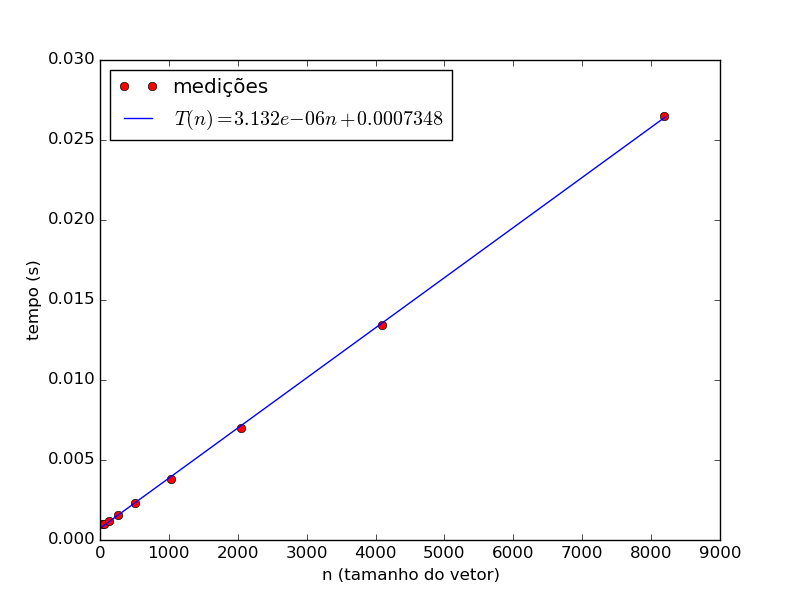
\includegraphics[scale=0.8]{../countingsort/imagens/countingsortQuaseDecresc500.png}
\caption{A análise do grafico para $2^{32}$ segue abaixo para countingsort}

Tendo a função $T(n) = 3.132\mathrm{e}-6*n-0.0007348$ e para o $n =2^{32}$, $T(2^{32}) = 13451.836836272$ 
\label{fig:countingsortQuaseDecresc500}
\end{figure}

\begin{figure}[ht]
\centering 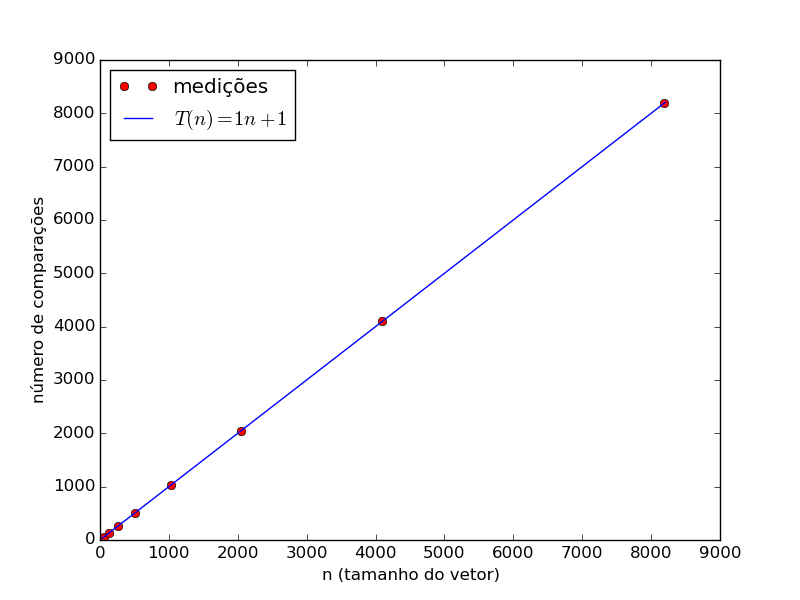
\includegraphics[scale=0.8]{../countingsort/imagens/countingsortQuaseDecresc501.png}
\caption{A análise do grafico para $2^{32}$ segue abaixo para countingsort}

Tendo a função $T(n) = n+1$ e para o $n =2^{32}$, $T(2^{32}) = 4294967297$ 
\label{fig:countingsortQuaseDecresc501}
\end{figure}


\clearpage
\clearpage
\addcontentsline{toc}{part}{Apêndice}
\appendix

\chapter{Arquivo ../countingsort/countingsort.py \label{ap:countingsort}}
\lstinputlisting[caption={../countingsort/countingsort.py \label{arq:countingsort}}]{../countingsort/countingsort.py}

\chapter{Arquivo ../countingsort/ensaio.py \label{ap:countingsortensaio}}
\lstinputlisting[caption={../countingsort/ensaio.py \label{arq:countingsortensaio}}]{../countingsort/ensaio.py}

\end{document}
